\chapter{Analysis and Results}


\section{2018 vdM scan program}



\section{Data analysis}



\section{Module selection}


\section{Background estimation}







\begin{table}[h!]
  \begin{center}
    \caption{Background mean value and SEM of each BCID for both SS periods .}
    \label{ss_per_bx}
    \begin{tabular}{|c | c | c | }
      \multicolumn{1}{c}{} & \multicolumn{1}{c}{\textbf{SS period I}} & \multicolumn{1}{c}{}  \\
      \hline
 \textbf{BCID}   & \textbf{Mean}   &  \textbf{SEM}\\
     \hline %\midrule[1.1pt]
      265 & 0.3111 & 0.0172\\
      \hline
      865 & 0.2732 & 0.0135\\ 
      \hline
      1780 & 0.3223 & 0.0187\\ 
      \hline
      2192 & 0.2875 & 0.0159\\ 
      \hline
      3380 & 0.3157 & 0.0162\\ 
      \hline
      \multicolumn{1}{c}{} & \multicolumn{1}{c}{} & \multicolumn{1}{c}{}\\
      \multicolumn{1}{c}{$\text{SSI}_{\text{Avg}}=$} & \multicolumn{1}{l}{$0.302 \pm 0.0073$} & \multicolumn{1}{c}{}\\
%      \multicolumn{1}{c}{} & \multicolumn{1}{c}{} & \multicolumn{1}{c}{}
    \end{tabular}
    \hspace{0.5cm}
    \begin{tabular}{|c | c | c | }
      \multicolumn{1}{c}{} & \multicolumn{1}{c}{\textbf{SS period II}} & \multicolumn{1}{c}{ }  \\
      \hline
 \textbf{BCID}   & \textbf{Mean}   &  \textbf{SEM}\\
     \hline %\midrule[1.1pt]
      265 & 0.3027 & 0.0148\\
      \hline
      865 & 0.297 & 0.0156\\ 
      \hline
      1780 & 0.304 & 0.0167\\ 
      \hline
      2192 & 0.2225 & 0.0114\\ 
      \hline
      3380 & 0.3064 & 0.0169\\ 
      \hline
      \multicolumn{1}{c}{} & \multicolumn{1}{c}{} & \multicolumn{1}{c}{}\\
      \multicolumn{1}{c}{$\text{SSII}_{\text{Avg}}=$} & \multicolumn{1}{l}{$ 0.287 \pm 0.0068$} & \multicolumn{1}{c}{}
    \end{tabular}   
  \end{center}
\end{table}


Table \ref{ss_per_bx} shows the mean en SEM values for each BCID for both SS periods and the average and error ($AvgErr= \sqrt{SEM_1^2+SEM_2^2+\cdots SEM_{N}}/N) $) per SS period. Having both average values of SS, the average and error is taken, being this the value applied as a background correction:  $ 0.29 \pm 0.005$.

\section{Corrections}
The PCC rates per NB4 are averaged per scan step (30s) and the uncertainty is calculated as the SEM. The following corrections are applied in the vdM FW:

\begin{enumerate}
\item Ghost and Satellite. Corrects for the presence of ghost and satellite spurious charges. This correction affects bunch currents. Satellite charges refers to charge in the colliding bunch crossing but not in the colliding RF bucket, while spurious charges refers to charge not in any nominally filled bunch slot.% 
% The satellite charges are measured by the FBCT, and the DCCT measurements integrate over all charges, thus include both type of contributions.  so a correction of the beam intensities is needed in order to obtain an accurate value. For the 2018 VdM fill, these contributions are measured using the LHC longitudinal density monitors [23, 24]. Ghost charge measurement is also performed using the beamgas imaging method [25] by comparing the beam-gas rates in beam-empty and empty-empty crossings at the LHCb interaction point (IP8).\\
%The correction data is taken and the correction is performed as $B_{1,2}*(1-ghos)$ and $B_{1,2}*(1-sat)x$
\item Background. Value estimated above is subtracted to the rates.% lumB = lum - bkg;  %  lumErrB = np.sqrt(lumErr**2 + bkgErr**2). Bkg value in the prev sect. is subtracted and the error is propahated as : sqrt
\item Orbit drift. The Orbit Drift (OD) correction is composed of two independent corrections: separation correction and a rate correction. OD separation aims at correcting for the orbit drift in the scanning direction and only affects beam separation.  OD rate aims at correcting for the orbit drift in the direction orthogonal to the scanning direction and only affects luminometer rate. The derived correction assumes that the beam overlap has a single gaussian shape. The correction reads the $\Sigma$ in the orthogonal direction from the previous correction.
%entry.lumiPerBX[bx] = [ rate * np.exp( ody**2 / (2*CS[bx]**2) ) for rate, ody in zip(entry.lumiPerBX[bx], OD_Y) ]
%entry.lumiErrPerBX[bx] = [ rateErr * np.exp( ody**2 / (2*CS[bx]**2) ) for rateErr, ody in zip(entry.lumiErrPerBX[bx], OD_Y) ]
%CS es en la ortogogonal y el od creo que es el de la OD sep.

\item Beam Beam. Corrects Beam Beam deflection (BB) that happens during bunch crossings at the collision point. The deflection is calculated and added to the nominal separation.
  %https://gitlab.cern.ch/bril/VdMFramework/-/blob/even_more_fits_aa/Code/dataPrep_corr/makeBeamBeamFile.py
  %import BB -> formula?

\item Dynamic Beta. The so-called dynamic-$\beta*$ effect, which accounts for the fact that each beam has a defocusing effect on the other. This effect is calculated using reference beam transport simulations that are scaled to the beam energies, the  $\beta ^{*}$ settings, and the measured intensities and convoluted beam widths. %Rate normalized? %correction_factor en framework. makedynfile y dyncoor.

\item Length Scale.  It applies a linear scaling to the beam separation to convert it from the "CMS scale" to the actual "physics scale". This correction is estimated by analyzing pp collision vertices reconstruced by the CMS tracker. %scaling but sepErr is 0...

\item Peak to peak. Corrects for error in peak calculation, when the scan does not cover the actual head-on collision of the beams. %peakToPeakFactor = np.exp( mean**2 / (2 * capSigma**2) );  peakToPeakFactorErr = peakToPeakFactor * mean / capSigma**3 * np.sqrt( capSigma**2 * meanErr**2 + mean**2 * capSigmaErr**2)

%https://gitlab.cern.ch/bril/VdMFramework/-/wikis/od-flag
\end{enumerate}


\section{van der Meer Scans and $\sigma_{vis}$ Results}

The measurements of PCC, beam separation and beam currents were plotted, fitted and corrected with the corrections described above. The fit model impleted is a guassian-like function: 

$$Poly\mathbf{2}G= P \cdot \Biggl[1+r_{2} \cdot \Biggl( \frac{x-\bar{x}}{\frac{\sigma}{1+r_{2}}} \Biggr)^{2}   \Biggr]\cdot \exp \Biggl[ - \frac{1}{2} \Biggl(  \frac{x-\bar{x}}{ \frac{\sigma}{1+r_{2}} }  \Biggr)^{2} \Biggr] $$

where $P$ is the peak value, $\bar{x}$ the mean, and $\sigma$ (standard deviation) and $r_{2}$ are fit parameters. This model will be referred as ``Poly2G''. Fig. \ref{vdM1_1780_XYscan} shows the fitted graphs of the first vdM scan pair for BCID 1780. Fig. \ref{vdM1_1780_XYscan_logy} shows the same graphs in logarithmic scale. Note that rates are normalized by the beam currents, which is a factor of eq. \ref{sigmavis_eq}  ($R(0,0)/N_{1}N_{2}$).

The rest of the BCIDs, vdM and imaging scans present a very similar behaviour. Fig \ref{chi2/ndof} shows a plot of the chi2/ndof for all the seven scan pairs, having a mean value of 2.23. In all cases the fits converged. The $\Sigma_{x,y}$  (referred also as CapSigma) and peak values were extracted from the fits to compute $\sigma_{vis}$. Fig \ref{capsigma_peak} shows $\Sigma_{x,y}$ and peak values for all scan pairs. As can be seen, both values reflects the fact that beam size increased over time in the $x$ dimension and decreased over time in the $y$ dimension.
\begin{center}
\begin{figure}[ht]
\centering
%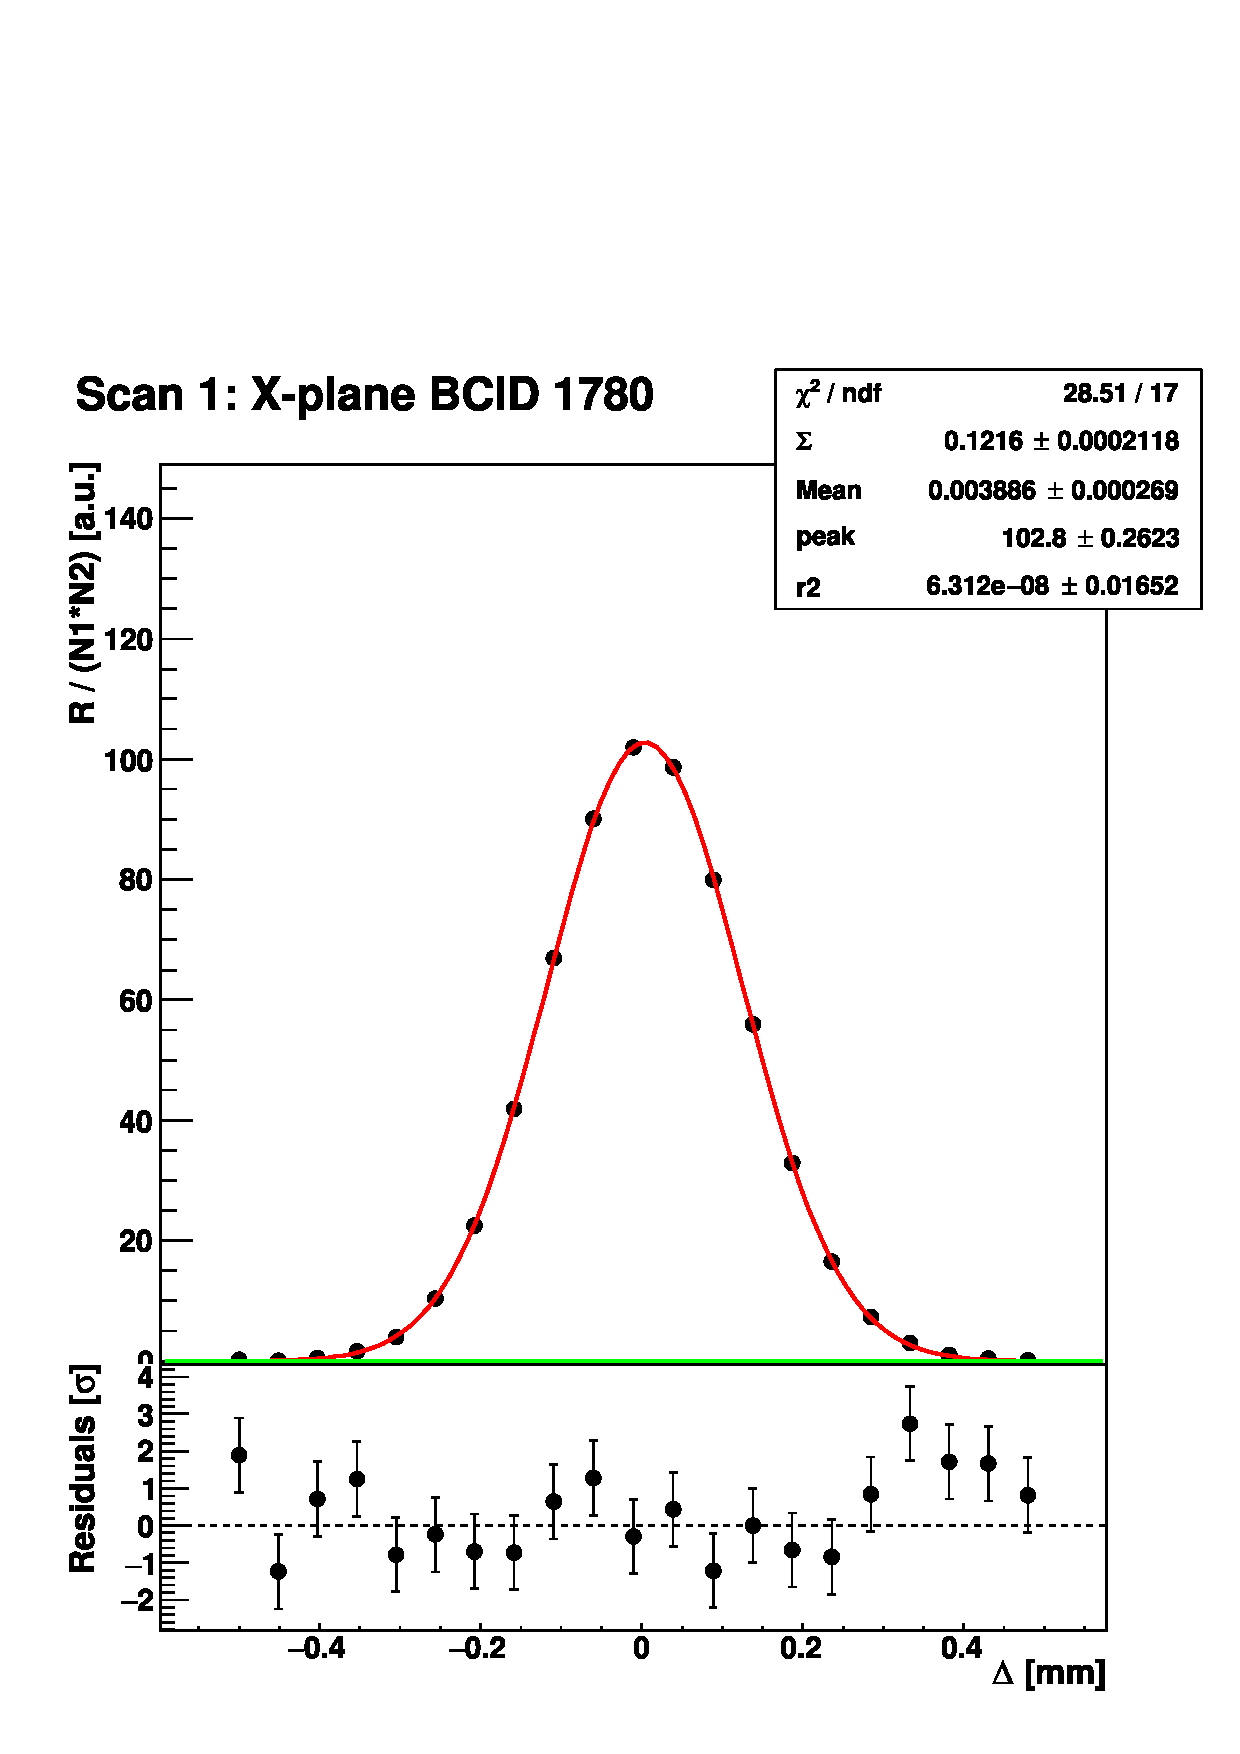
\includegraphics[width=.45\textwidth]{Chapter4/plots/vdM1_BX1780_XScan_v2.pdf}
%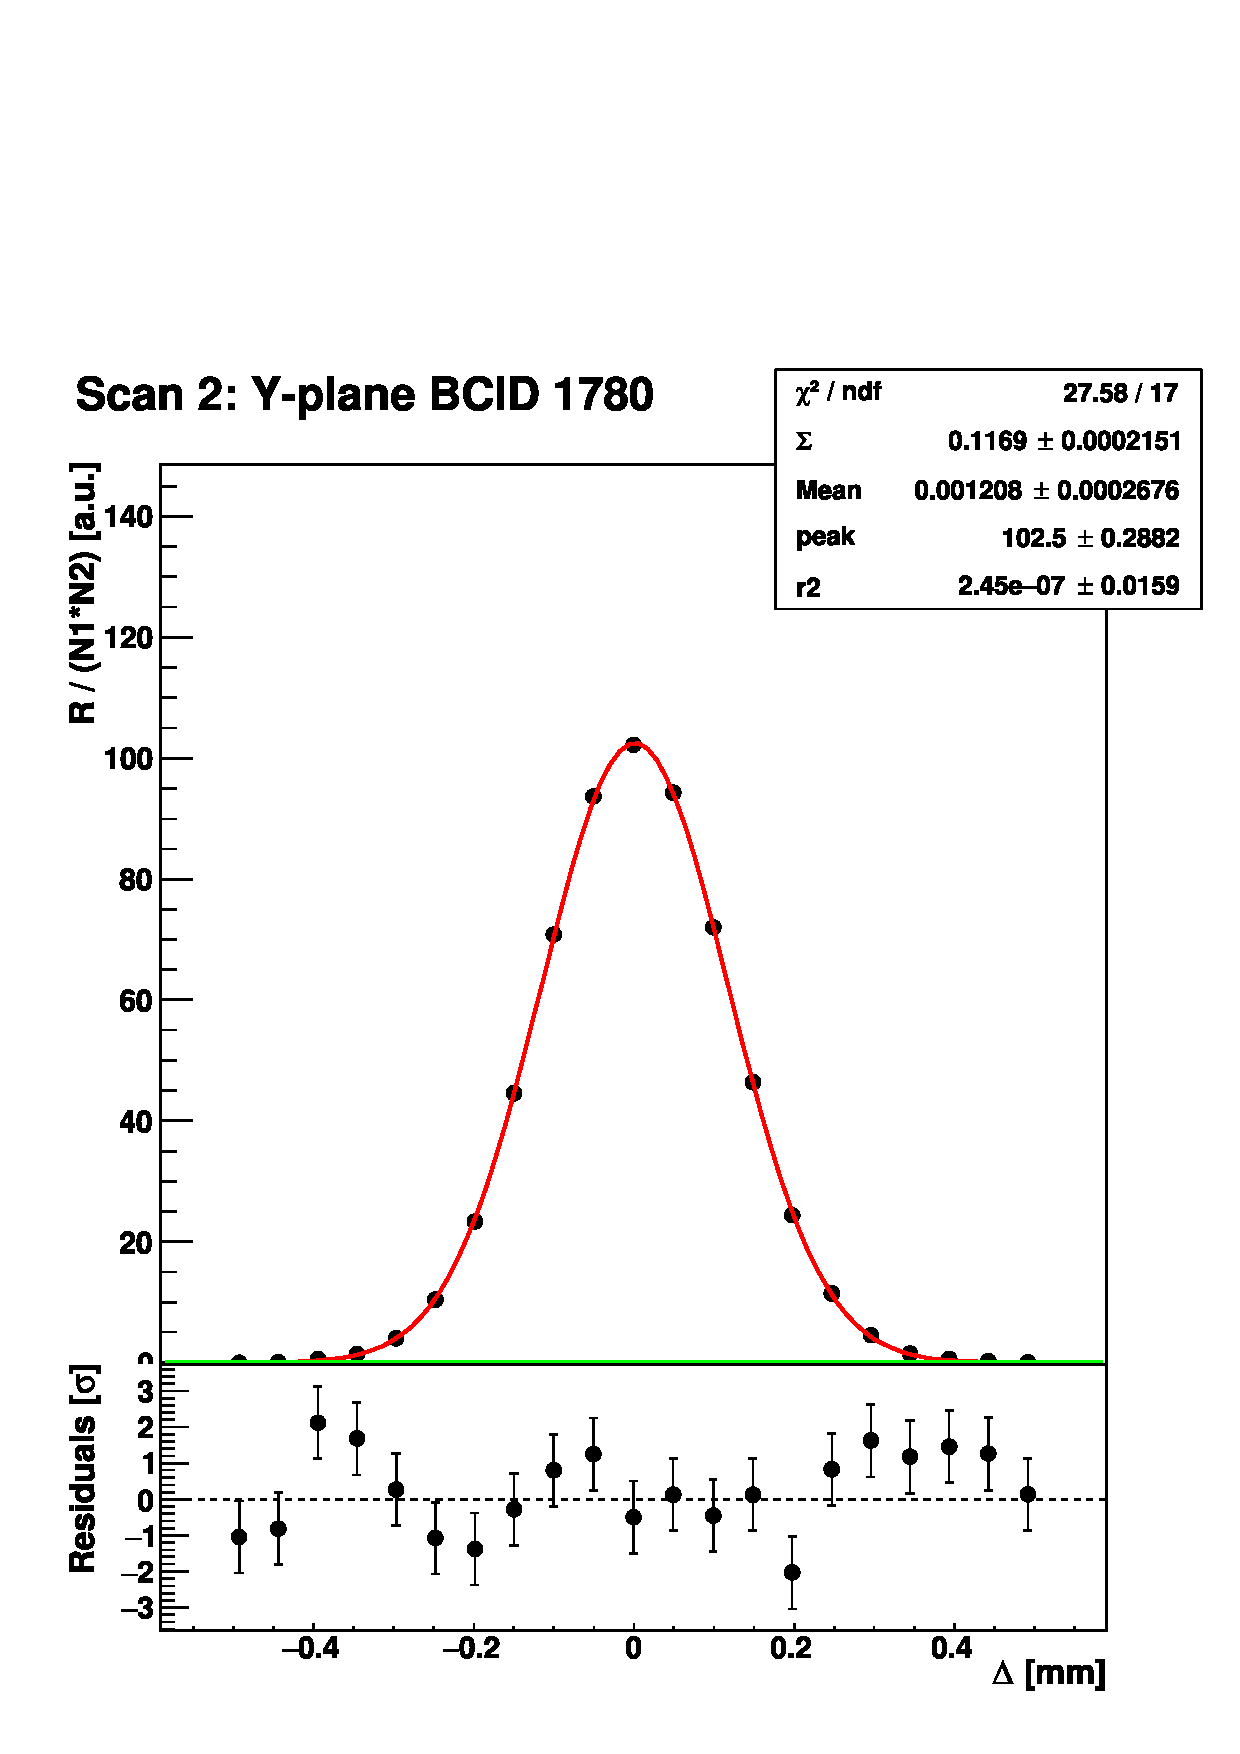
\includegraphics[width=.45\textwidth]{Chapter4/plots/vdM1_BX1780_YScan_v2.pdf}\\
%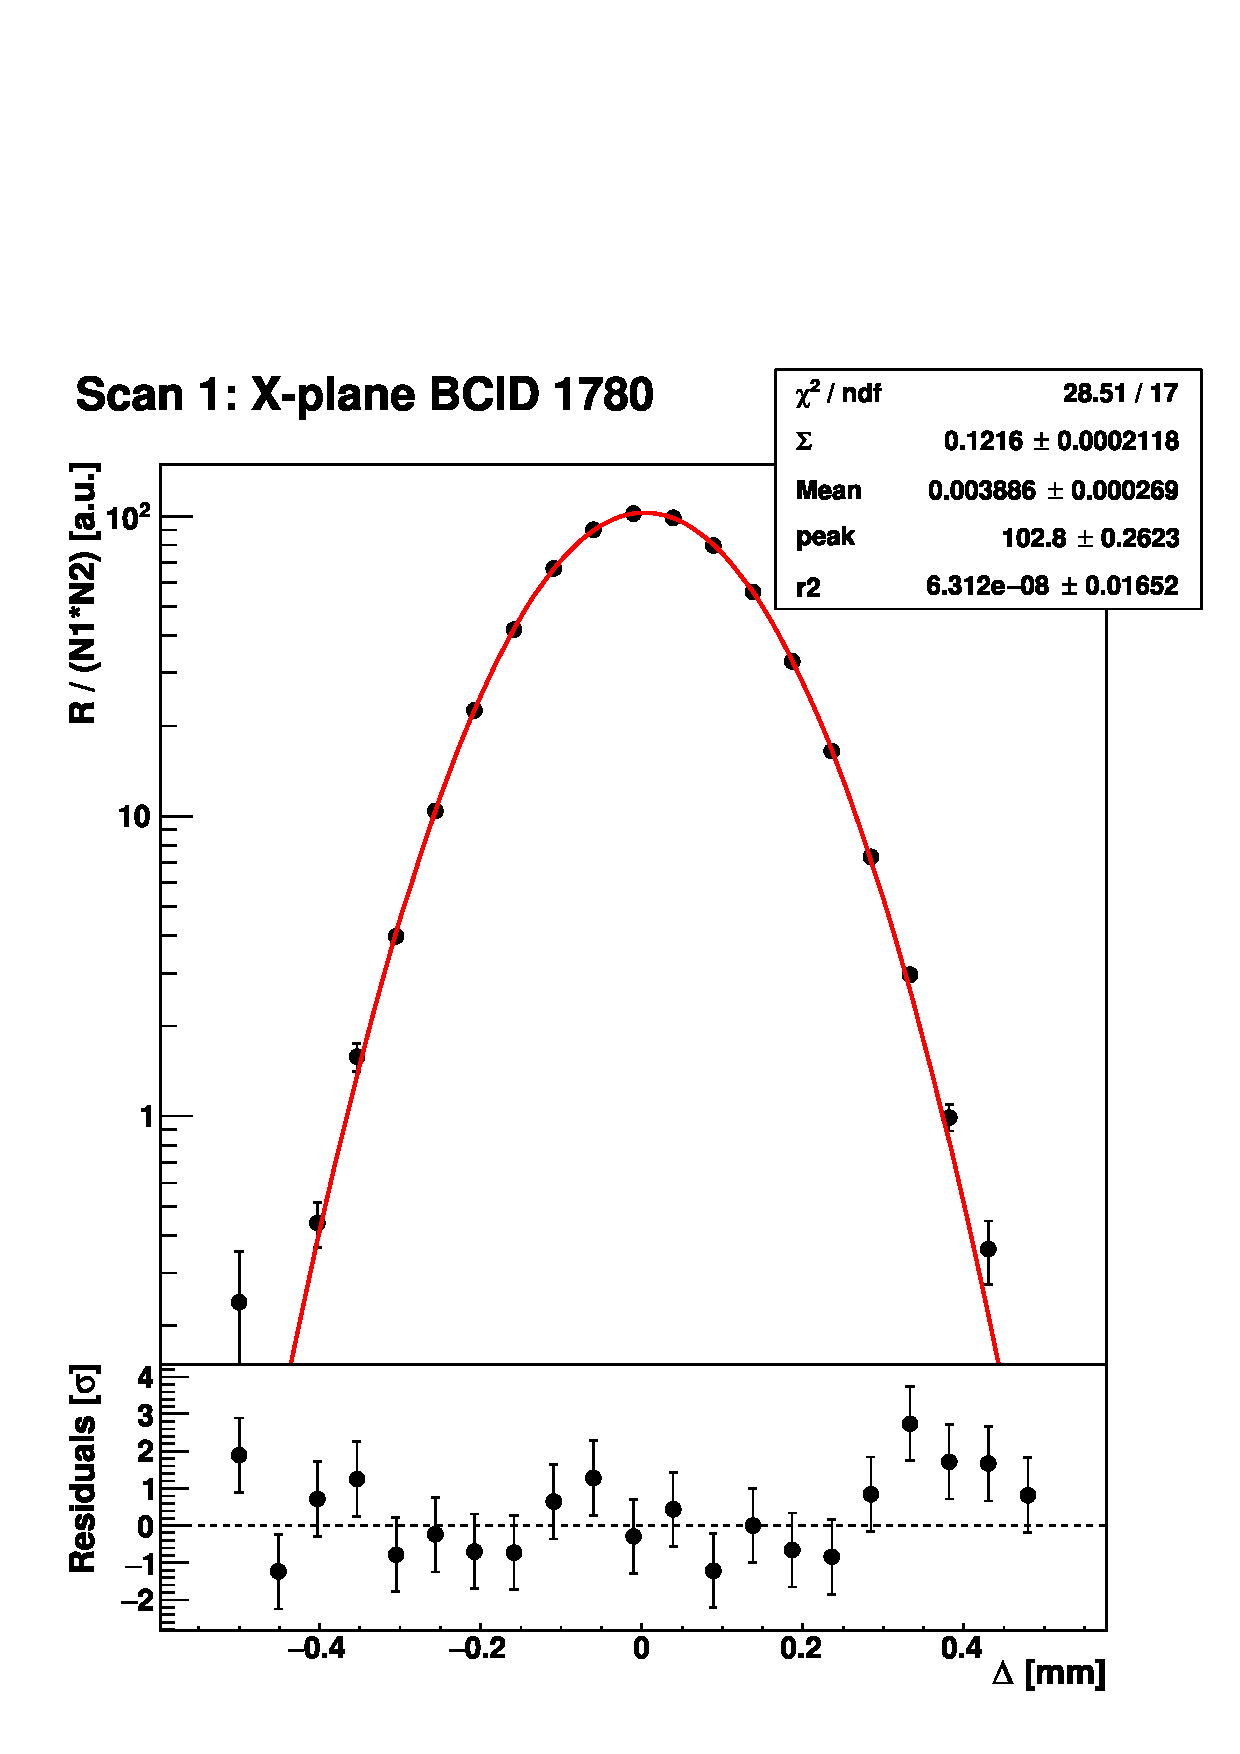
\includegraphics[width=.45\textwidth]{Chapter4/plots/vdM1_BX1780_XScan_v2_LOGY.pdf}
%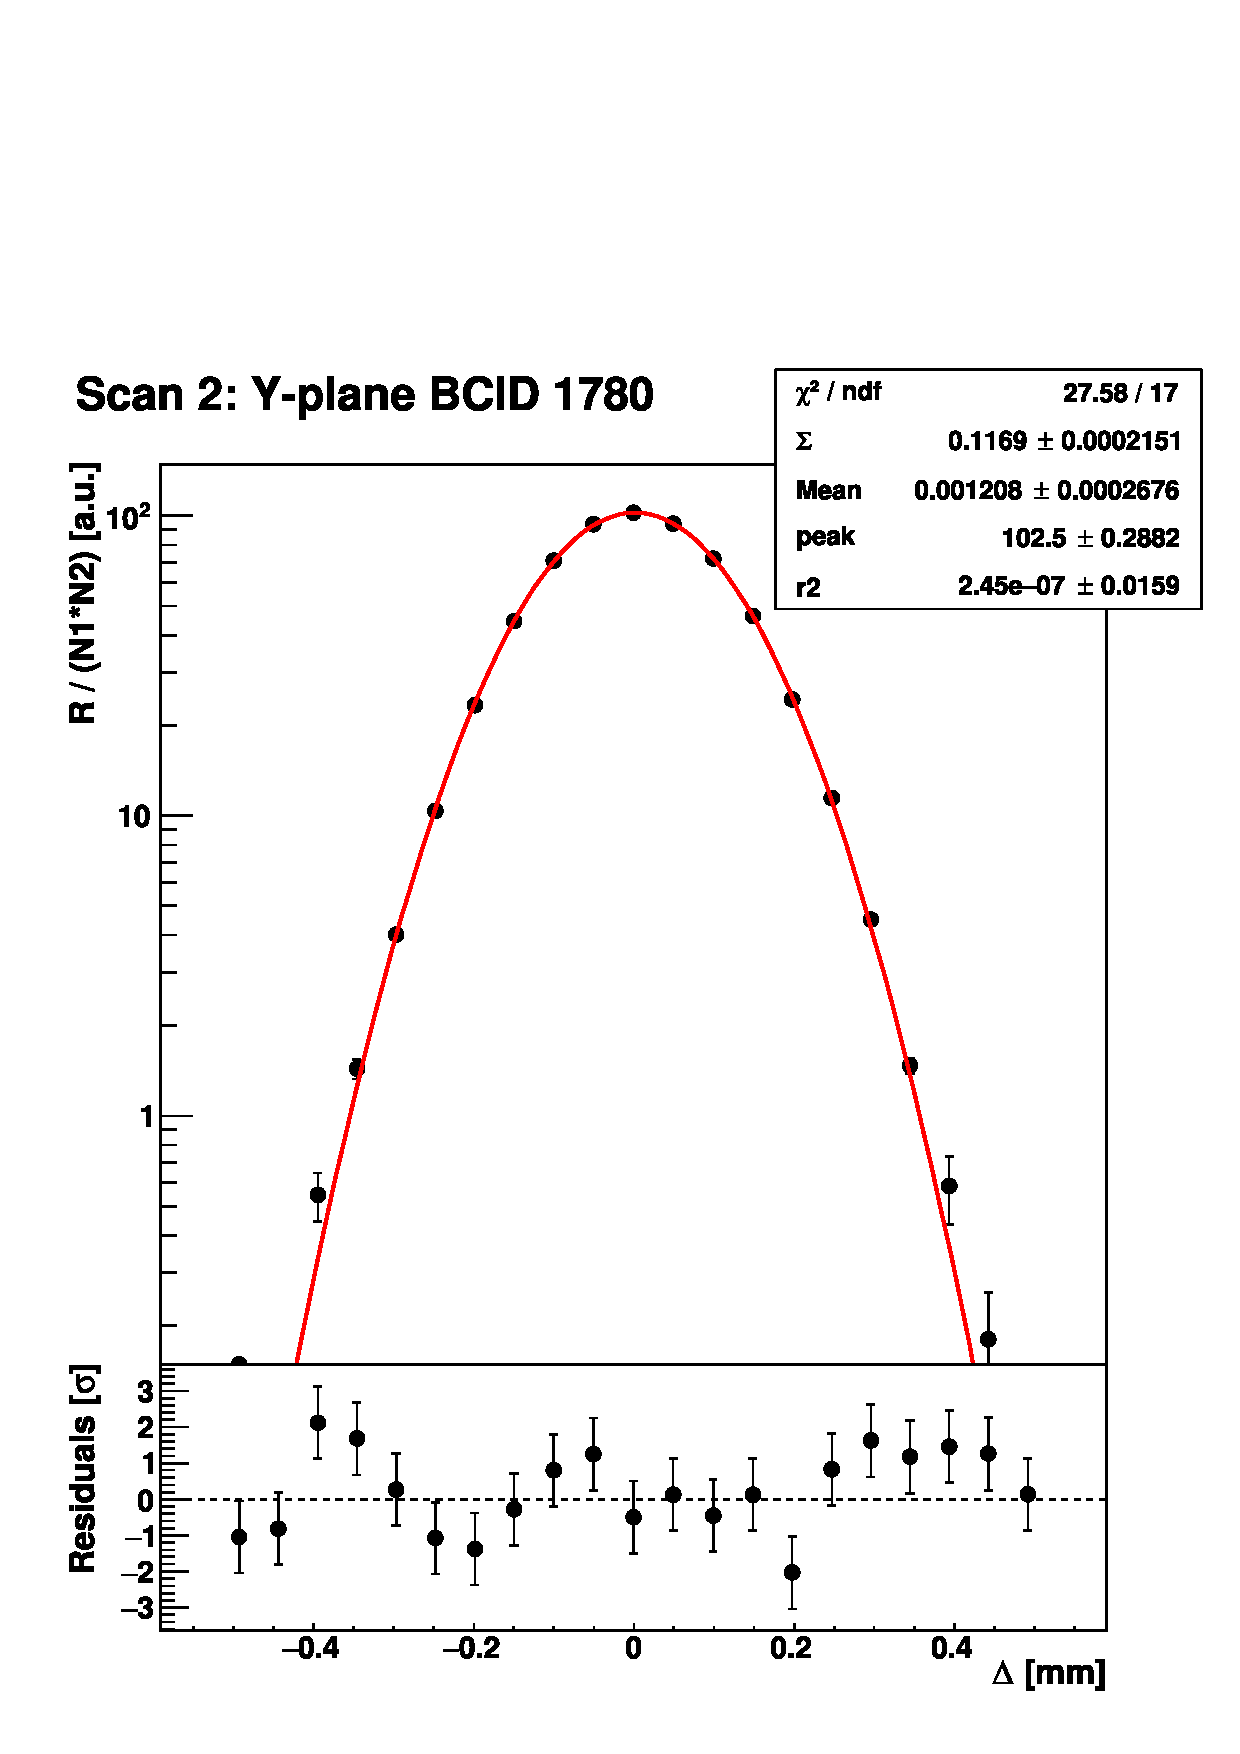
\includegraphics[width=.45\textwidth]{Chapter4/plots/vdM1_BX1780_YScan_v2_LOGY.pdf}
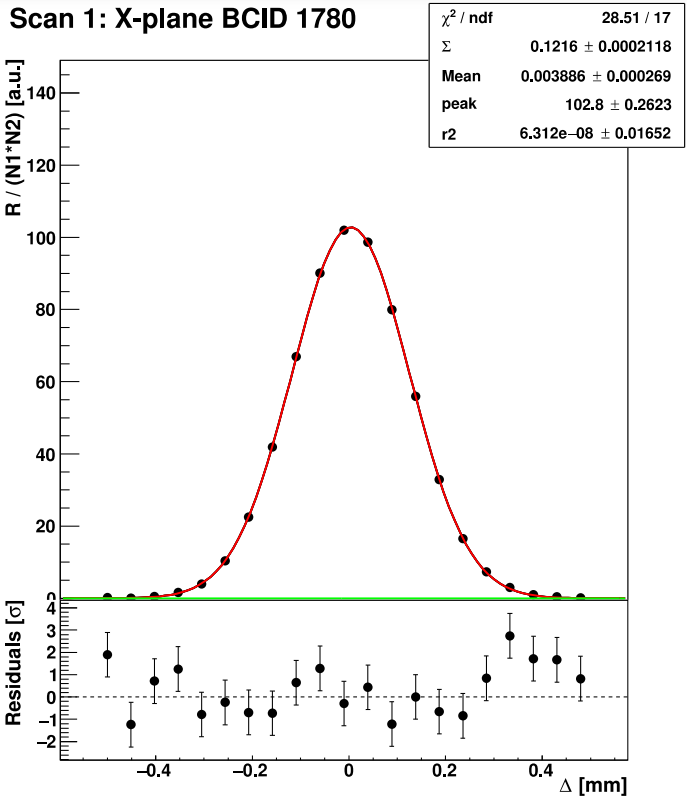
\includegraphics[width=.38\textwidth]{Chapter4/plots/xscan.png}
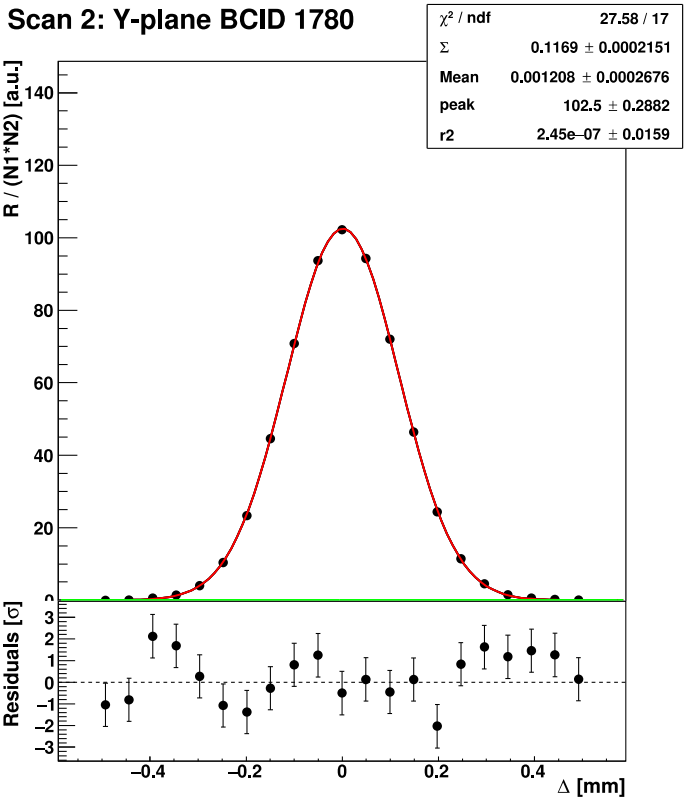
\includegraphics[width=.38\textwidth]{Chapter4/plots/yscan.png}\\
%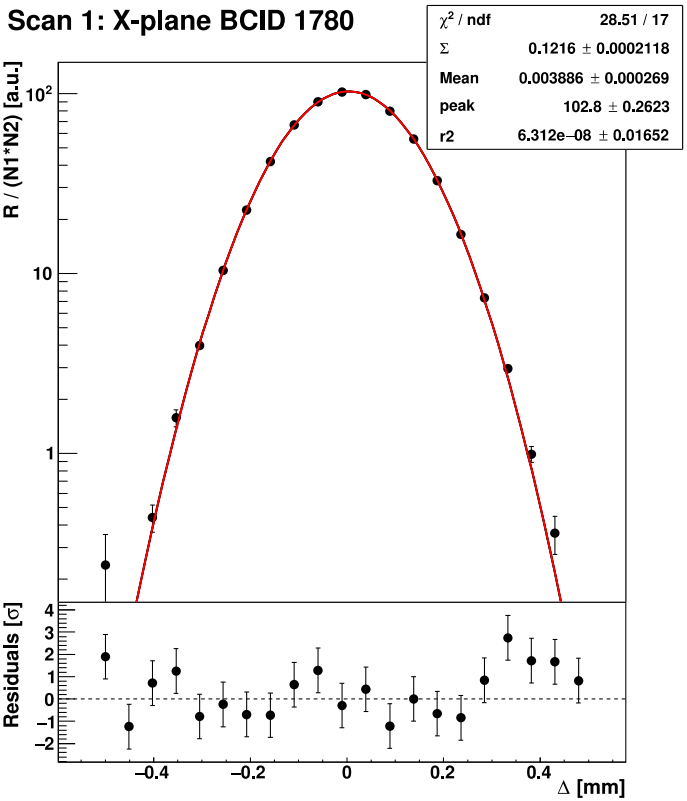
\includegraphics[width=.39\textwidth]{Chapter4/plots/xscan_logy.png}
%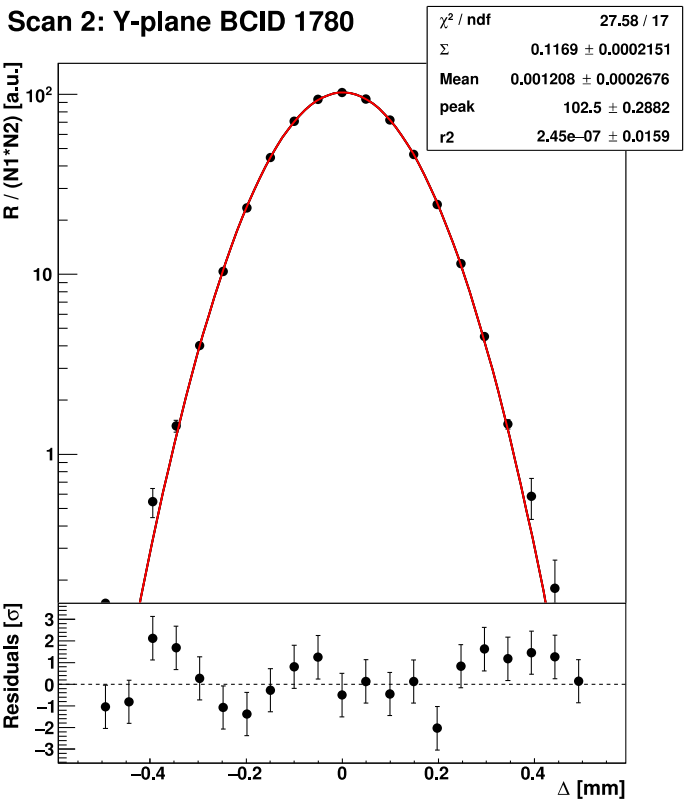
\includegraphics[width=.39\textwidth]{Chapter4/plots/yscan_logy.png}
\caption[vdM1 BCID 1780 (linear scale)]{Normalized rates and the resulting fitted curves with the Poly2G fit model (see text) as a function of
  the beam separation ($\Delta$) for BCID 1780 for X (left) and Y (right) scan for the first vdM scan. Background subtraction and the corrections described in the previous section have been applied to the raw data before the fit.}
\label{vdM1_1780_XYscan}
\end{figure}
\end{center}

\begin{center}
\begin{figure}[ht]
\centering
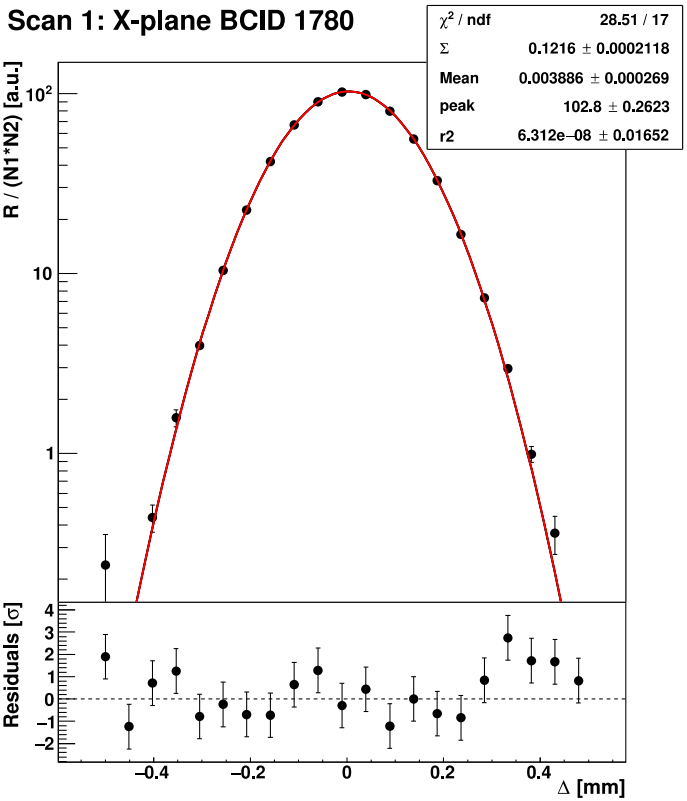
\includegraphics[width=.39\textwidth]{Chapter4/plots/xscan_logy.png}
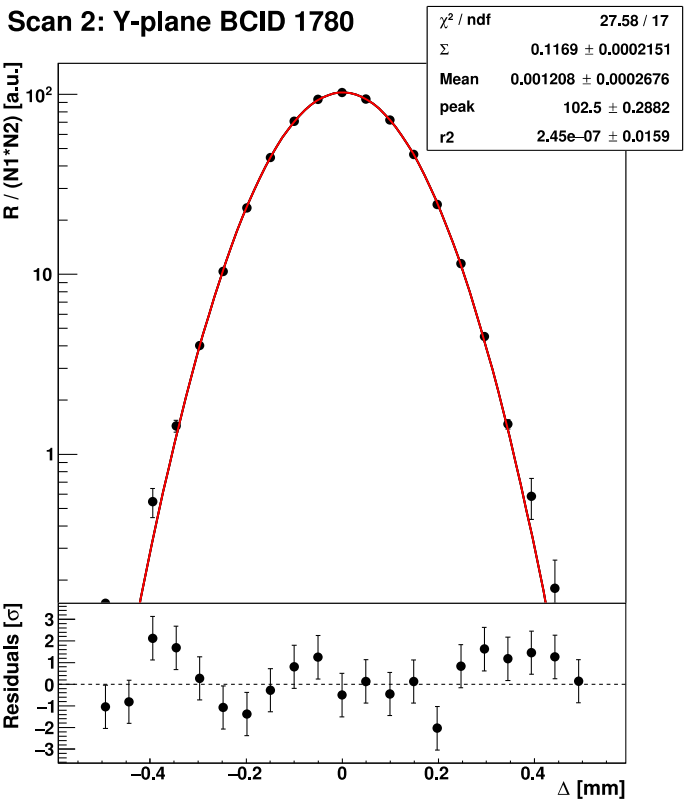
\includegraphics[width=.39\textwidth]{Chapter4/plots/yscan_logy.png}
\caption[vdM1 BCID 1780 (logarithmic scale)]{Fig. \ref{vdM1_1780_XYscan} in logarithmic scale.}
\label{vdM1_1780_XYscan_logy}
\end{figure}
\end{center}

\begin{center}
  \begin{figure}[ht]
    \centering
    \includegraphics[scale=.20]{Chapter4/plots_thesis/chi2_Poly2G.png}
    \caption[chi2/ndof for all scan pairs]{ chi2/ndof for all the scan pairs. Vertical blue lines divide the X (left) and Y (right) scans. In each scan, the BCIDs follow the same order: 265, 865, 1780, 2192, 3380.} %[ https://indico.cern.ch/event/1099207/contributions/4625225/attachments/2351526/4011953/PCC_Stability_Study_23_11_2021.pdf]
    \label{chi2/ndof}
  \end{figure}
\end{center}

\begin{center}
  \begin{figure}[ht]
    \centering
    \includegraphics[width=.49\textwidth]{Chapter4/plots_thesis/CapSigma_Poly2G.png}
    \includegraphics[width=.49\textwidth]{Chapter4/plots_thesis/peak_Poly2G.png}
    \caption[$\Sigma$ and peak values for all scan pairs]{$\Sigma$ (left) and Peak values (right) extracted from the fitted graph to compute $\sigma_{vis}$.  Vertical blue lines divide the X (left) and Y (right) scans. In each scan, the BCIDs follow the same order: 265, 865, 1780, 2192, 3380.} %[ https://indico.cern.ch/event/1099207/contributions/4625225/attachments/2351526/4011953/PCC_Stability_Study_23_11_2021.pdf]
    \label{capsigma_peak}
  \end{figure}
\end{center}
%Eos results path:
%/eos/user/j/jmorenoc/Results_v1/NewVeto/Period_B/Tests_Poly246G/No_Limits_Poly246G_SuperG/Output/plots_Poly2G/CapSigma_Poly2G.png
The $\sigma_{vis}$ of each BCID is computed from the fit results parameters showed in previous section ($\Sigma_{x,y}$ and peak) using \ref{sigmavis_eq} with  $R(0,0)=(Peak_{x}+Peak_{y})/2$; $Peak_{x,y}$ values are already normalized so \ref{sigmavis_eq} is rewritten as $\sigma= 2\pi \Sigma_{x} \Sigma_{y} (Peak_{x}+Peak_{y})/2$.\\
Fig \ref{sigmavis_perbcid} shows  $\sigma_{vis}$ per BCID for all the scans. The error on $\sigma_{vis}$ is assigned as $\sigma_{vis\text{Err}}= 2 \pi \sqrt{ (\Sigma_{y} \cdot R \cdot \Sigma_{x\text{Err}})^{2} + (\Sigma_{x} \cdot R \cdot \Sigma_{y \text{Err}})^{2} + (\Sigma_{x} \Sigma_{y} R_{\text{Err}})^{2} }$.\\ %The mean value is 9232.26 mb  with a standard deviation (bunch spread) of  44.33 mb (0.48 \%).
Fig \ref{sigmavis_perscan} shows $\sigma_{vis}$ per Scan, which corresponds to the weighted average of the five BCIDs with the weight as $1/\sigma_{vis\text{Err}}^{2}$. The error is assigned as $1/\sqrt{\sum \frac{1}{\sigma_{vis\text{Err}}^{2}}}$.\\

%\begin{equation*}
%\frac{1}{\sqrt{\sum_{i}^{N}\frac{1}{\sigma Err^{2}_{i}}}}
%\end{equation*}
  
%and the systematic uncertainty as

%$$\sqrt{RMS^{2}-stat^{2}}$$
\begin{center}
  \begin{figure}[ht]
    \centering
    \includegraphics[scale=.25]{Chapter4/plots_thesis/Poly2G_xsec.png}
    \caption[$\sigma_{vis}$ per BCID for all scans]{ $\sigma_{vis}$ per BCID for all the scans.  In each scan the BCIDs follow the same order: 265, 865, 1780, 2192, 3380.} %[ https://indico.cern.ch/event/1099207/contributions/4625225/attachments/2351526/4011953/PCC_Stability_Study_23_11_2021.pdf]
    \label{sigmavis_perbcid}
  \end{figure}
\end{center}

The $\sigma_{vis}$ per scan are averaged and assigning the error in the same way described above, giving a value of $9229 \pm 8 \text{(stat.)} \text{mb}$.\\
As can be seen in  Fig \ref{sigmavis_perscan}  (and Fig \ref{sigmavis_perbcid}), there is some systematic variation in $\sigma_{vis}$ from scan to scan, being the first vdM scan lower than the rest of the scans. The systematic error is assigned as $\sqrt{RMS^{2}-stat^{2}}$. \\
Therefore the $\sigma_{vis}$ value is

\begin{equation}
\sigma_{vis} = 9229 \pm 8 \text{(stat.)} \pm 28 \text{(syst.)} \text{ mb} .
\end{equation}

This value is higher than the previously reported in ref. \cite{pas_18}: 5982 mb, which corresponds to a different selection of modules in the pixel detector. In the previous result, 1069 modules were removed, whereas the value of 9229 mb corresponds to 802 modules removed; the rate of pixel clusters is proportional to the number of modules.

\begin{center}
  \begin{figure}[ht]
    \centering
    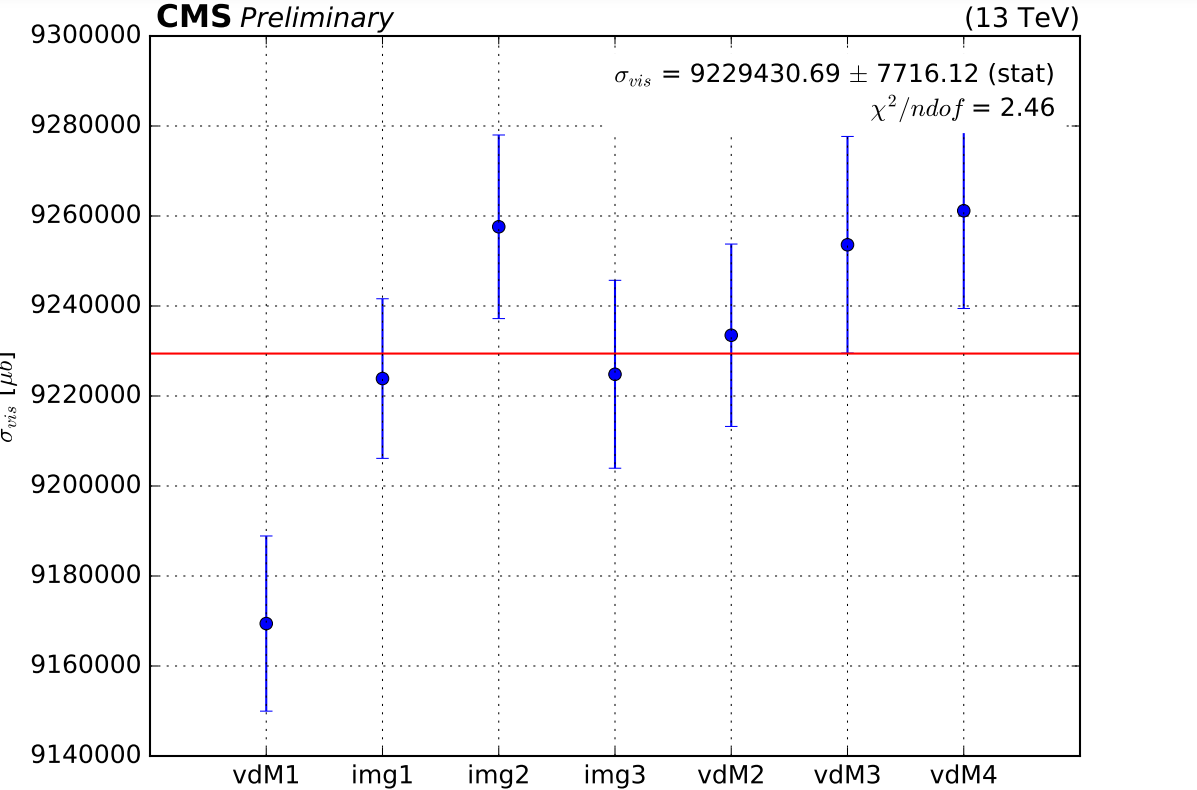
\includegraphics[scale=0.37]{Chapter4/plots/xsec_perscan_v2.png}
    \caption[$\sigma_{vis}$ per Scan]{ $\sigma_{vis}$  per scan.} %[ https://indico.cern.ch/event/1099207/contributions/4625225/attachments/2351526/4011953/PCC_Stability_Study_23_11_2021.pdf]
    \label{sigmavis_perscan}
  \end{figure}
\end{center}
